% 1. Какую систему Вы изучаете в Вашей диссертационной работе? Что является объектом исследования.
% 2. Каково назначение Вашей системы?
% 3. Какова цель исследования системы? Где она может быть использована?
% 4. Частью какой надсистемы является изучаемая система?
% 5. Из каких подсистем состоит система?
% 6. Какие задачи решают подсистемы в составе Вашей системы?
% 7. Сформулируйте кратко сценарий функционирования системы.

В качесте системы для исследования я обозначил структуру приложения предназначенного для интеграции в в плагинную систему. Мною проанализирована предметная область, сформулированы ограничения на компоненты системы и предложена формулировка ее описания в виде графовой модели. Полученная модель позволяет оценивать суммарный объем требований, включенный в поставку при заданном объеме минимально необходимых для включения требований. Это применимо для вычисления коэффициента простоя подразделений компании поставщика вовлеченных в пост продажное обслуживание.

Как говорилось ранее, для описания системы был проведен анализ предметной области и сформулирован минимальный объем ограничений сущностей предметной области для описания математической модели. Так, математическая модель состоит из следующих сущностей, к которым применены ограничения:
\begin{enumerate}
    \item сущности классифицированы:
    \begin{enumerate}
        \item поставка, включающая конкретный перечень плагинов;
        \item плагины пригодные для интеграции в плагинную систему;
        \item файлы исходного кода распределенные по плагинам;
        \item функциональные зависимости между файлами исходного кода и плагинами;
        \item требования реализованные в файлах исходного кода
    \end{enumerate}
    \item один файл может реализовывать одно или несколько требований;
    \item одно требование может быть реализовано в одном или нескольких файлах;
    \item один файл не может быть включен в несколько плагинов;
    \item файлы имеют зависимости друг на друга, в том числе и циклические;
    \item плагины так же имеют зависимости друг на друга: если в плагин включены файлы, зависящие от файлов, расположенных в другом плагине, то первый плагин зависим от второго;
    \item циклические зависимости между плагинами запрещены.
\end{enumerate}

Принципиальная схема приведена на рисунке \ref{fig:graph}

\begin{figure}[H]
    \centering
    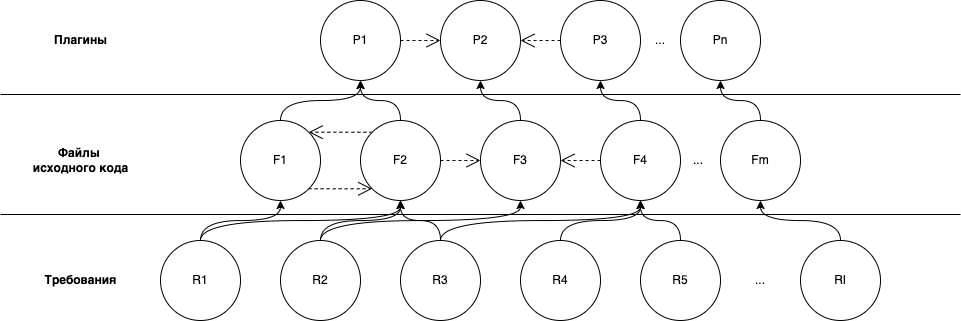
\includegraphics[width=1\textwidth]{graph}
    \caption{Система с приведенными подсистемами}
    \label{fig:graph}
\end{figure}

Рассматриваемая система является частью жизненного цикла ПО. Начиная от формирования изначального потенциально возможного перечня требований оформленных в виде ТЗ и заканчивая формированием поставки под нужды конкретного потребителя.

Так, имеется IT продукт с реализованным набором требований заданных в ТЗ. Требования реализованы в файлах исходного кода, которые в свою очередь распределены по плагинам, из которых можно выполнить поставку. Предположим, что заказчику потребны не все реализованные требования, а часть из них. Тогда необходимо сформировать поставку, в которую потребные требования войдут точно, но еще и войдут требования, которые ему не потребны. Отношение непотребных требований к общему числу требований я называю качеством поставляемого функционала, от качества зависит эффективность использования IT продукта заказчиком.

Схема с отображением проблемы приведена на рисунке \ref{fig:life_circle}

\begin{figure}[H]
    \centering
    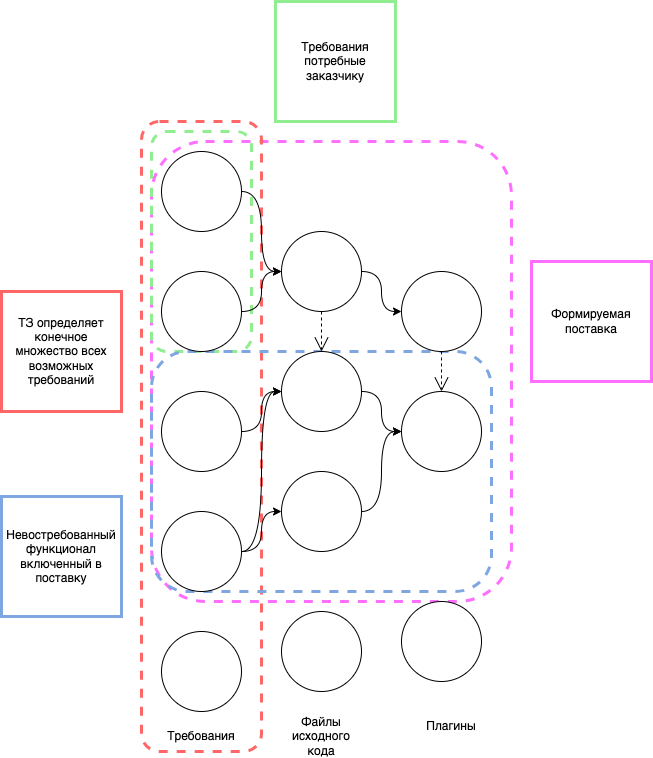
\includegraphics[width=1\textwidth]{life_circle}
    \caption{Формирование поставки по потребным заказчику требованиям}
    \label{fig:life_circle}
\end{figure}